\section{ハードウェア}
\subsection{駆動系}
 今回のRCRでは,去年と同様のモータ,エンコーダ,駆動輪を使用することにした.以下にこれらの性能を示す.
今回の課題では自己位置推定が重要になってくるため,ロータリーエンコーダをギヤードモータにつけずに,車軸に取り付けるようにした.モータの動力はギアを介してタイヤに伝える.これによって万が一ギヤがかみ合わなかったときにもタイヤの回転を読み取ることができる.
また,本大会で採用した機構は独立二輪機構である.独立二輪機構は,四輪車のようにステアリング操作が必要なく,モータの出力を制御することで旋回することができ,また内輪差もないため,旋回を多く行うRCRでは有効である.ただし,独立二輪機構は直線安定性に劣るため,ロータリーエンコーダを用いてソフトウェアで制御していく.

\begin{description}
 \item[【ギヤードモータ 3633K10】] \mbox{} \\ 
	    最大回転数:372 [rpm] (無負荷時,印加電圧 8.0[V]) \\
	    定格電圧:24[V] \\
	    定格トルク:0.5 [kg·cm] (最大効率時)        
 \item[【ロータリーエンコーダ RE30E-500-213-1】] \mbox{} \\
	    インクリメンタル型 \\
	    パルス / 回転:500 \\
	    電源電圧:5~12 [V] ギヤを介して,ギヤを介して,
 \item[【駆動輪】] \mbox{} \\
	    直径64 [mm] \\
	    厚み 24.5 [mm]
\end{description}


\begin{figure}[b]
 \begin{center}
  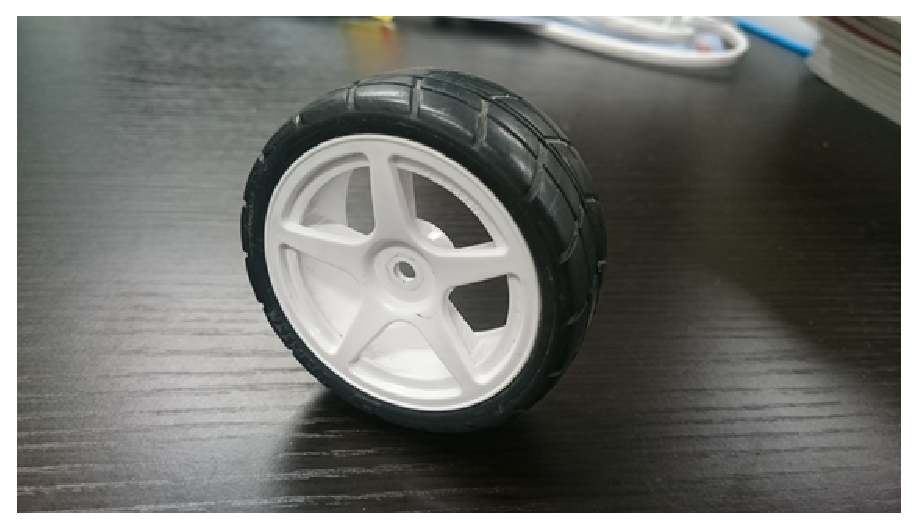
\includegraphics[scale=.5]{../kuwano/picture/picture1.eps}
  \caption{駆動輪}
 \end{center}
\end{figure}


\begin{figure}[H]
 \begin{center}
  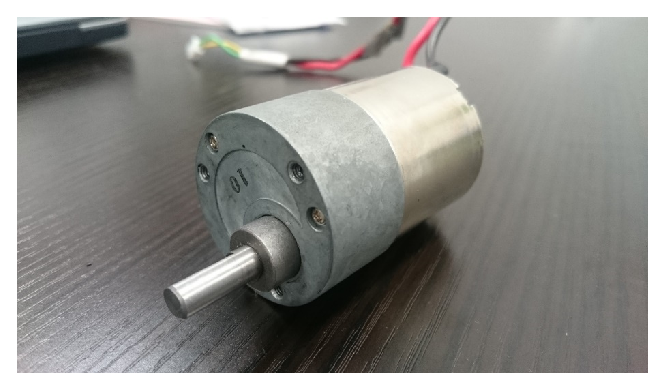
\includegraphics[scale=.7]{../kuwano/picture/picture2.eps}
  \caption{ギヤードモータ3633K10}
 \end{center}
\end{figure}

\begin{figure}[H]
 \begin{center}
  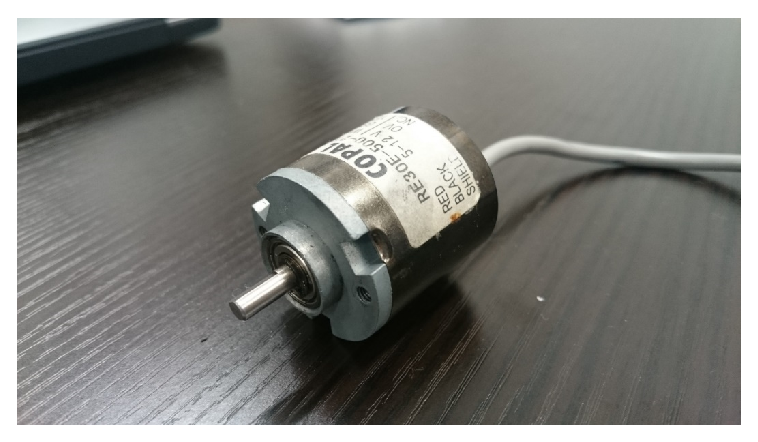
\includegraphics[scale=.7]{../kuwano/picture/picture3.eps}
  \caption{ロータリーエンコーダ RE30E-500-213-1}
 \end{center}
\end{figure}



\subsection{車体の設計}
 3D CADソフト Inventorを用いて設計したロボットカーの全体図を図\ref{fig:robocar}に示す.設計の際に工夫した点は,センサの位置を対象物(ポール)をとらえやすい位置に置いたことである.「対象物をとらえやすい位置」はまだ実際に試走してみないと分からないが,センサの高さはスペーサーのサイズを変えることで容易に修正することができるため,ロボカーが対象物をとらえるのに最適な位置を決めることができる.
また,車体を八角形にすることにより,ロボカーがその場で旋回するときに不意にポールに衝突するのを防ぐことができる.
階層の構成は,駆動系を一階,センサやバッテリー類など,あまり触ることのないものを二階,マイコンやアーム部分を三階に設置した.ロボカーの一階,二階,三階部分を図\ref{fig:1F},図\ref{fig:2F},図\ref{fig:3F}に示す.

\begin{figure}[hb]
 \begin{center}
  \includegraphics[scale=.3]{../kuwano/picture/picture4.eps}
  \caption{ロボカー全体図}
  \label{fig:robocar}
 \end{center}
\end{figure}

\begin{figure}[H]
 \begin{center}
  \includegraphics[scale=.3]{../kuwano/picture/picture5.eps}
  \caption{一階部分}
  \label{fig:1F}
 \end{center}
\end{figure}

\begin{figure}[H]
 \begin{center}
  \includegraphics[scale=.3]{../kuwano/picture/picture6.eps}
  \caption{二階部分}
  \label{fig:2F}
 \end{center}
\end{figure}

\begin{figure}[H]
 \begin{center}
  \includegraphics[scale=.3]{../kuwano/picture/picture7.eps}
  \caption{三階部分}
  \label{fig:3F}
 \end{center}
\end{figure}
